As described in \cref{sec-hw-early-evolution}, the GPU hardware architecture has undergone a drastic development, and still is.
This section presents the GPU hardware architecture as a conceptual GPGPU architecture.
The architecture is presented from a GPU computing point of view, meaning that some elements which are only used for graphical purposes are not included.

%TODO Evt. tilføj Flynn's taxonomy (Hvis ikke Mathias introducere.)

The GPU hardware architecture consists of three main blocks categories:
\begin{itemize}
	\item Streaming Multiprocessors (SMs)
	\item Streaming Processors (SPs) 
	\item Memory (Local, Shared \& Global)
\end{itemize}

On a high level, the GPU can be described as an array of \textit{N} SMs, each consisting of \textit{M} cores (SPs). 
The number of SMs contained in GPUs varies a lot, from small GPUs only containing a single SM, to the newest Nvidia architecture \textit{Tesla V100} containing 84 SMs.
The number of SMs, and thereby the number of SPs, contained in the GPU enables more tasks to be processed at the same time or a single task to be processed faster if enough parallelism is implemented for this given task. 



\begin{figure}[ht]
	\centering
	\fbox{
		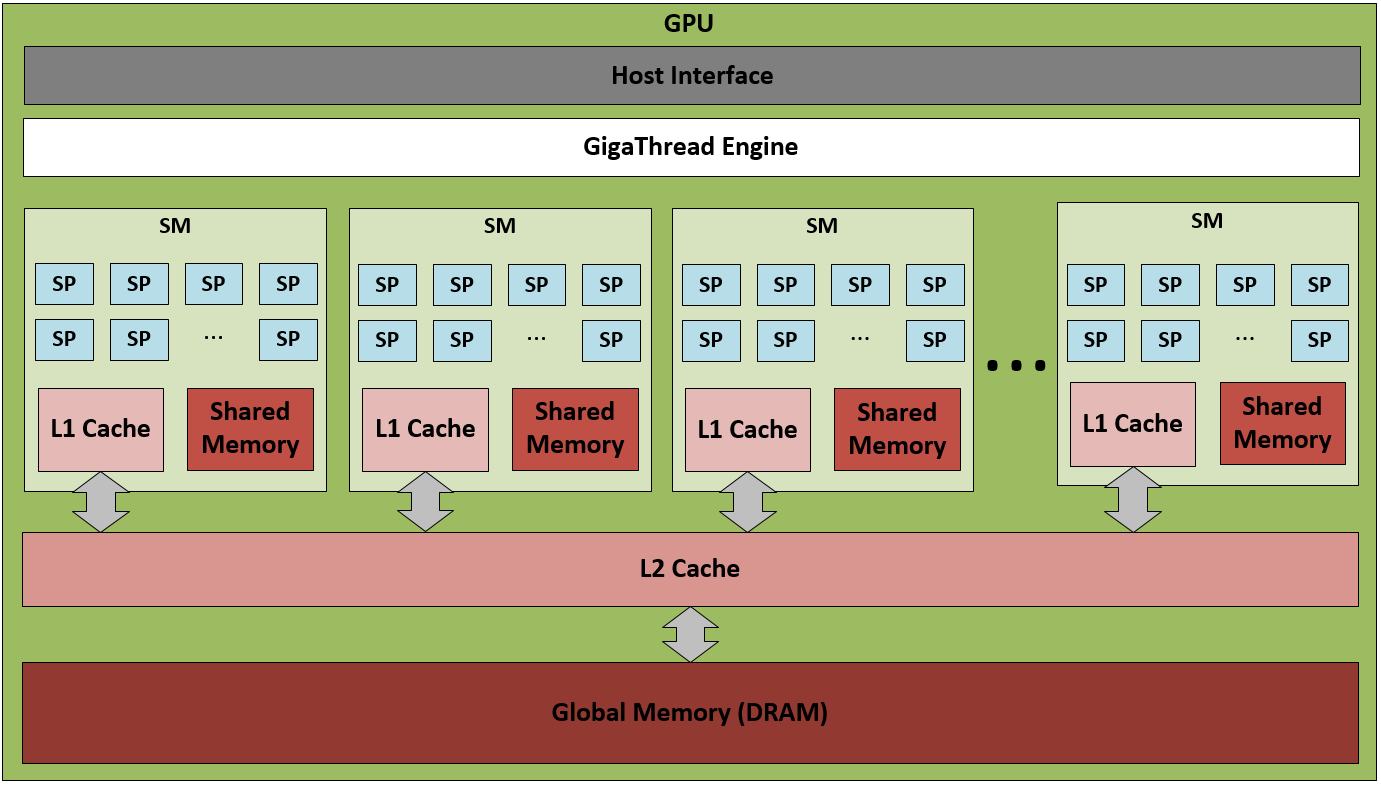
\includegraphics[width=1\textwidth]{figs/hw/hw-gpu}}
	\caption{Conceptual GPGPU hardware architecture}
	\label{fig:hw-gpu}
\end{figure}